\begin{figure}[htb!]
\centering
\begin{tabular}{ccc}
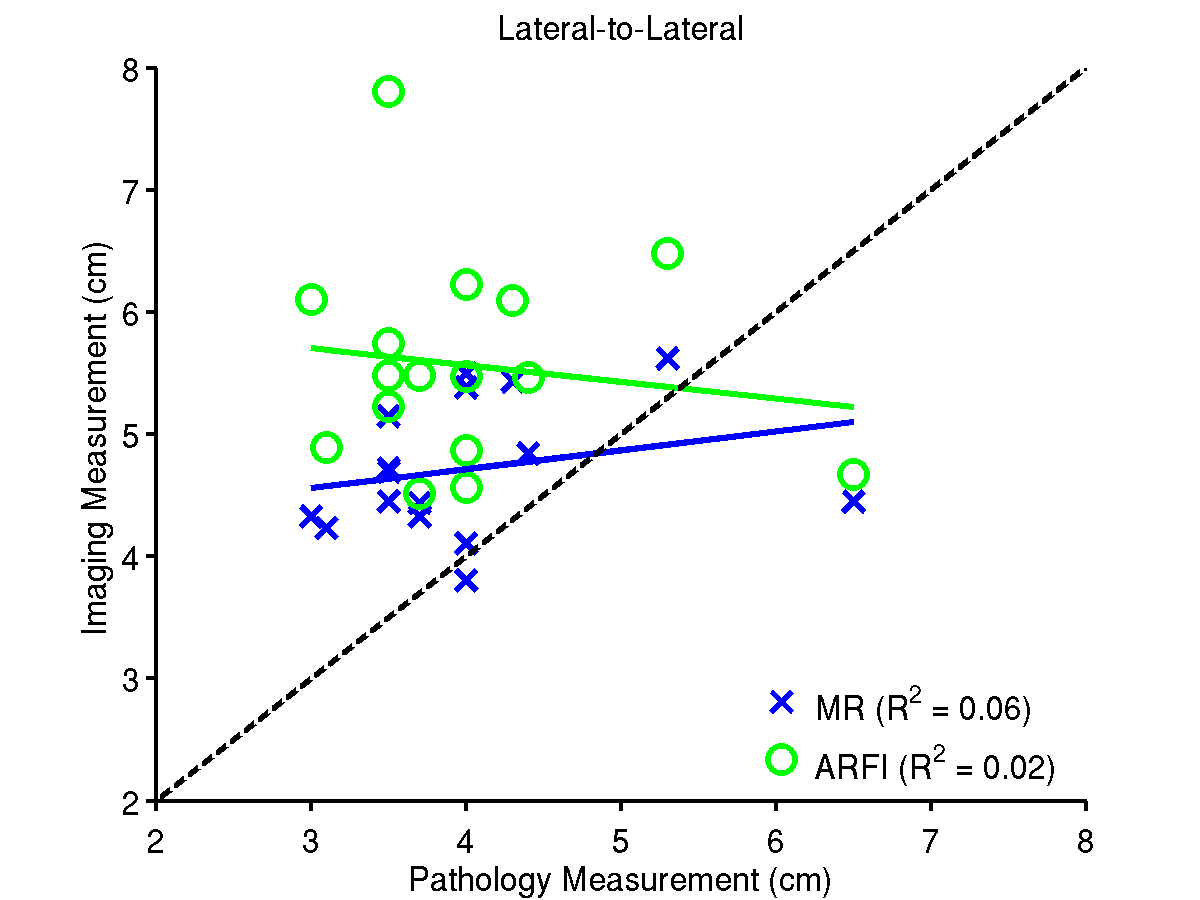
\includegraphics[width=0.3\linewidth]{figs/Lateral-to-Lateral} &
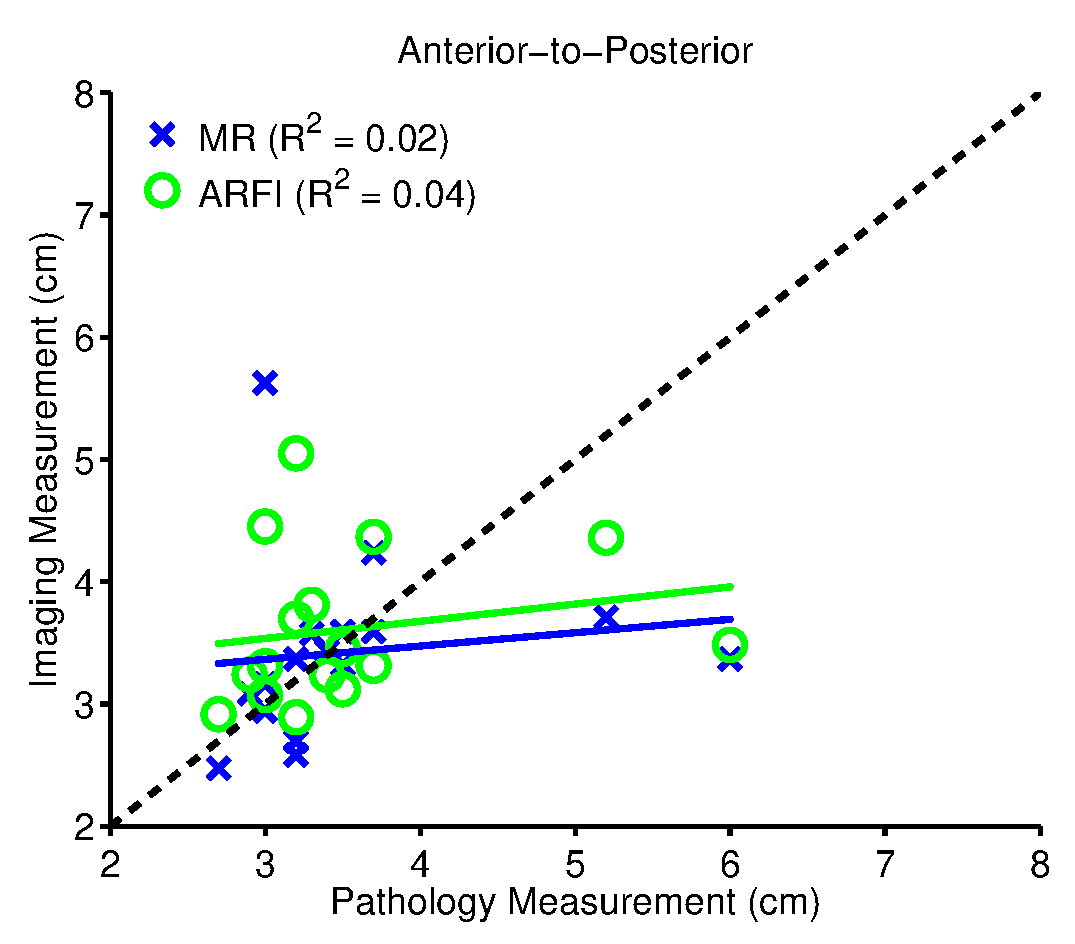
\includegraphics[width=0.3\linewidth]{figs/Anterior-to-Posterior} &
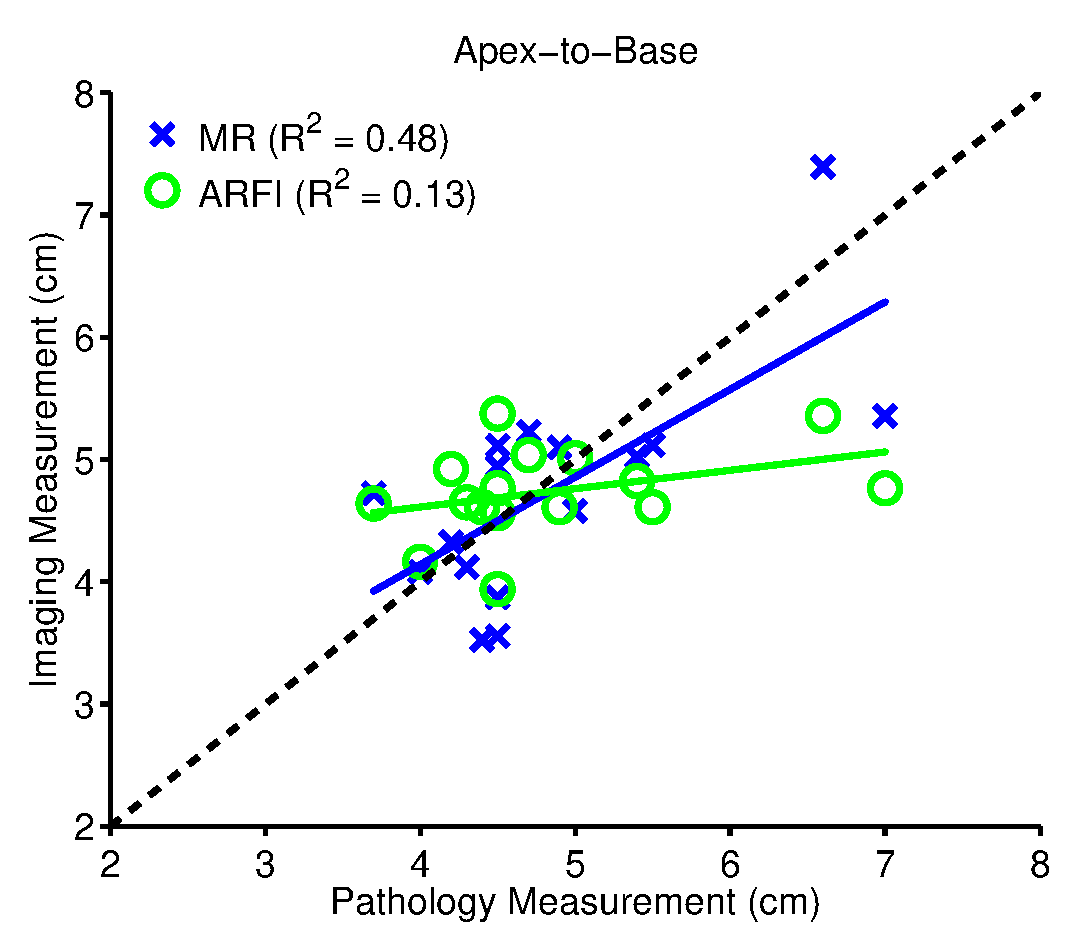
\includegraphics[width=0.3\linewidth]{figs/Apex-to-Base} \\
(a) & (b) & (c) \\
\end{tabular}
\caption{Measurements of the prostate dimensions along the three standard
anatomic axes: lateral-to-lateral (a), anterior-to-posterior (b) and
apex-to-base (c).  The correlation between the imaging axis measurements and
pathology was performed for each orientation.  The black dashed-line represents
the projection of perfectly-correlated measurements between imaging and
patholoy.  Notice that there is no correlation between imaging and pathology in
the lateral-to-lateral and anterior-to-posterior axes, with a general
over-estimation of the lateral-to-lateral axis in the imaging.  The MR
estimation of the apex-to-base dimension showed moderate correlation with
pathology, with the ARFI image apex-to-base approximation having an overall
underestimation in this orientation.  The over-/under-estimation of each imaging modality relative to gross pathology is summarized in Table~\ref{tab:mr_arfi_path_axes}.}
\label{fig:mr_arfi_path_axes} 
\end{figure}
